\documentclass[12pt,a4paper]{article}
\usepackage{algorithm, algpseudocode, amsmath, amssymb, amsthm, bm, csquotes, emf, empheq, geometry, graphicx, hyperref, listings, mhchem, multirow, siunitx, slashbox, subcaption, upgreek}
\usepackage[italicdiff]{physics}
\usepackage[section]{placeins}
\usepackage[justification=centering]{caption}
\usepackage[column=O]{cellspace}
\usepackage[extrafootnotefeatures]{xepersian}
\hypersetup{colorlinks=true, urlcolor=cyan}

\title{تمرین سری ده دینامیک غیرخطی و آشوب}
\author{صالح شاملو احمدی}
\date{۱۷ اردیبهشت ۱۴۰۲}

\settextfont{Yas}
\linespread{1.2}

\setlength\cellspacetoplimit{4pt}
\setlength\cellspacebottomlimit{3pt}
\newcommand{\multlinecell}[1]{\begin{tabular}[c]{@{}c@{}}#1\end{tabular}}

\newcommand{\qfrac}[2]{\left(\frac{#1}{#2}\right)}
\newcommand{\fsqrt}[2]{\sqrt{\frac{#1}{#2}}}
\newcommand{\ddfrac}[2]{{\displaystyle\frac{\displaystyle #1}{\displaystyle #2}}}
\newcommand{\pdvc}[3]{\qfrac{\partial #1}{\partial #2}_{#3}}
\newcommand{\dbar}{{d\mkern-7mu\mathchar'26\mkern-2mu}}
\newcommand*{\defeq}{\mathrel{\vcenter{\baselineskip0.5ex \lineskiplimit0pt
			\hbox{\scriptsize.}\hbox{\scriptsize.}}}
	=}

\newtheorem{theorem}{قضیه}
\newtheorem{lemma}{لم}
\renewcommand\qedsymbol{$\blacksquare$}

\begin{document}
	\maketitle
	\section{مسئله \lr{8.1.15}}
	\begin{subequations}
		\begin{empheq}[left=\empheqlbrace]{align}
			\dot{n}_A &= (p + n_A) n_{AB} - n_A n_B \\
			\dot{n}_B &= n_B n_{AB} - (p + n_A) n_B \label{typo} \\
			n_{AB} &= 1 - (p + n_A) - n_B
		\end{empheq}
	\end{subequations}
	اشتباه تایپی سؤال مربوط به معادله \eqref{typo} است که در آن جمله دوم
	$-(p + n_A) n_{AB}$
	چاپ شده. این جمله باید به شکل اول باشد چون تعدادی که از معتقدان $B$ کم می‌شود، متناسب با تعداد معتقدان خود $B$ است
	و به دسته بی‌طرف $AB$ ربطی ندارد.
	\subsection{\lr{a}}
	\begin{itemize}
		\item{جمله اول رابطه $\dot{n}_A$ (جمله $(p + n_A) n_{AB}$): متناسب با تعداد کل معتقدان $A$ و دسته بی‌طرف $AB$،
			برهم‌کنش بین $A$ و $AB$ داریم که نتیجه آن افزایش تعداد معتقدان غیرمتعصب $A$ است.}
		\item{جمله دوم رابطه $\dot{n}_A$ (جمله $-n_A n_B$): متناسب با تعداد معتقدان غیرمتعصب $A$ و تعداد معتقدان $B$،
			برهم‌کنش بین $A$ و $B$ به شکلی داریم که $B$ قانع‌کننده و $A$ قانع‌شونده باشد
			که نتیجه آن افزایش تعداد دسته بی‌طرف $AB$ و کم شدن از معتقدان غیرمتعصب $A$ است.}
		\item{جمله اول رابطه $\dot{n}_B$ (جمله $n_B n_{AB}$): متناسب با تعداد معتقدان $B$ و دسته بی‌طرف $AB$،
			برهم‌کنش بین $B$ و $AB$ داریم که نتیجه آن افزایش تعداد معتقدان $B$ است.}
		\item{جمله دوم رابطه $\dot{n}_B$ (جمله $-(p + n_A) n_B$): متناسب با تعداد کل معتقدان $A$ و تعداد معتقدان $B$،
		برهم‌کنش بین $A$ و $B$ به شکلی داریم که $A$ قانع‌کننده و $B$ قانع‌شونده باشد
		که نتیجه آن افزایش تعداد دسته بی‌طرف $AB$ و کم شدن از معتقدان $B$ است.}
	\end{itemize}
	\subsection{\lr{b}}
	\begin{figure}[h!]
		\centering
		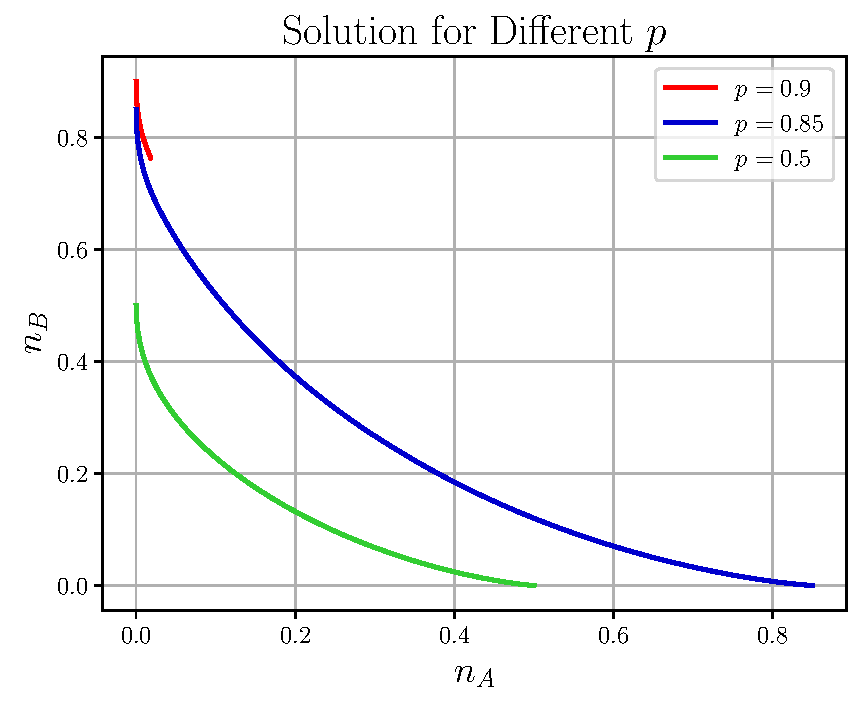
\includegraphics[width=\linewidth]{fig/8.1.15.solution.pdf}
		\caption{حل تحول سیستم برای $p$های مختلف}
	\end{figure}
	\begin{figure}[h!]
		\centering
		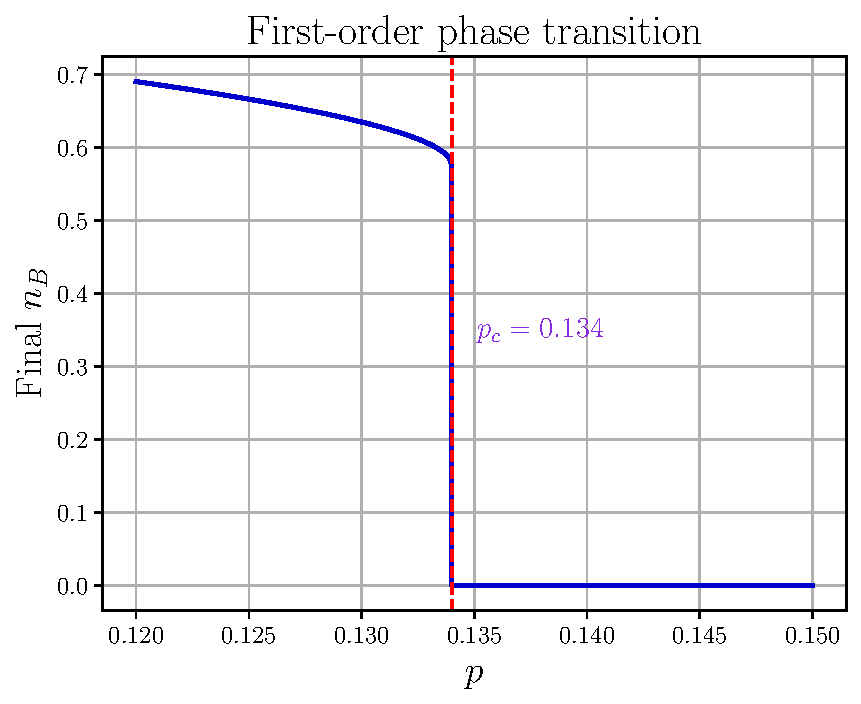
\includegraphics[width=\linewidth]{fig/8.1.15.bifurcation.pdf}
		\caption{دوشاخگی واقع در $p_c\approx1.134$ که منجر به یک گذار فاز مربته اول می‌شود.}
	\end{figure}
	\FloatBarrier
	\subsection{\lr{c}}
	\begin{subequations}
		\begin{empheq}[left={\dot{n}_B=0\implies\empheqlbrace}]{align}
			n_B &= 0 \\
			n_{AB} &= p + n_A \implies n_B = 1 - 2p - 2n_A
		\end{empheq}
	\end{subequations}
	\begin{subequations}
		\begin{empheq}[left={\dot{n}_A=0\implies\empheqlbrace}]{gather}
			n_A = 1-p;\quad n_B = 0 \\
			3n_A^2 + (4p - 1)n_A + p^2 = 0 \implies n_A = \frac{1-4p\pm\sqrt{4p^2-8p+1}}{6}
		\end{empheq}
	\end{subequations}
	بنابراین نقاط ثابت برابرند با
	\begin{subequations}
		\begin{empheq}[left=\empheqlbrace]{align}
			\qty(n_A^*, n_B^*) &= (1-p, 0), \\
			\qty(n_A^{*'}, n_B^{*'}) &= (\frac{1-4p\pm\sqrt{4p^2-8p+1}}{6}, 1-\frac{1+2p\pm\sqrt{4p^2-8p+1}}{6}).
		\end{empheq}
	\end{subequations}
	نقاط $n^{*'}$ وقتی با هم برابر می‌شوند که
	\begin{equation}
		4p^2-8p+1 = 0 \xRightarrow{0 < p < 1} p = 1 - \frac{\sqrt{3}}{2},
	\end{equation}
	بنابراین در این $p$ دوشاخگی داریم.
	
	برای اینکه نشان دهیم در $p$ بزرگ‌تر از $p_c = 1 - \flatfrac{\sqrt{3}}{2} $ تحت هر شرایطی جمعیت متعصب
	معتقد به $A$ در نهایت همه را معتقد به $A$ می‌کنند، باید نشان دهیم در این مقدار $p$، نقطه ثابت $\qty(n_A^*, n_B^*)$
	پایدار است. بدین منظور، ژاکوبی را در این نقطه محاسبه می‌کنیم.
	\begin{equation}
		J_{(n_A, n_B)} = \mqty(1-2(p + n_A + n_B) & -2(p + n_A) \\ -2n_B & 1 - p - 2(n_A + n_B)) \implies
	\end{equation}
	\begin{equation}
		J_{(n_A^*, n_B^*)} = \mqty(-1 & -1 \\ 0 & p-1) \implies \lambda_1 = -1,\quad\lambda_2 = p-1
	\end{equation}
	بنابراین هر دو ویژه مقدار ژاکوبی در این نقطه در هر شرایطی منفی هستند، پس این نقطه ثابت پایدار است
	و در غیاب دو نقطه دیگر تمام مسیرها به آن ختم می‌شوند.
	\subsection{\lr{d}}
	دوشاخگی از نوع زین--گره است چون دو نقطه ثابت نزدیک هم می‌شوند و همدیگر را نابود می‌کنند.
	\section{مسئله \lr{8.2.9}}
	\subsection{\lr{a}}
	\begin{figure}[h!]
		\centering
		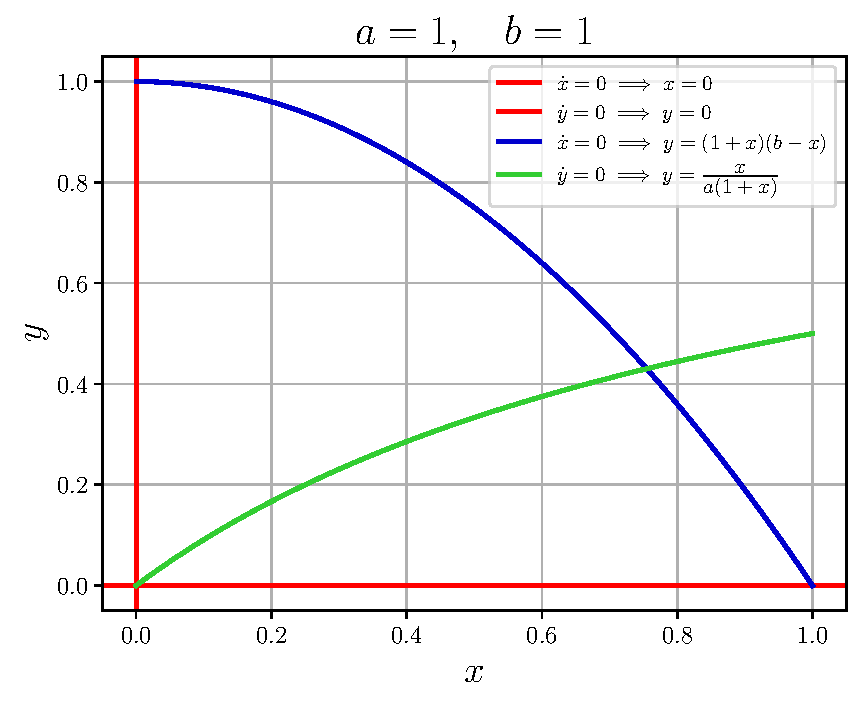
\includegraphics[width=\linewidth]{fig/8.2.9.nullclines}
		\caption{خم‌های پوچ}
	\end{figure}
	با توجه به نمودار، سه نقطه ثابت داریم:
	$(0, 0)$، $(b, 0)$
	و یک نقطه که محل تقاطع خم‌های $y=\flatfrac{x}{a(1+x)}$ و $y=(1+x)(b-x)$ است. حال پایداری نقاط ثابت را
	با محاسبه ژاکوبی بررسی می‌کنیم.
	\begin{equation}
		J = \mqty(b-\ddfrac{y}{(1+x)^2}-2x & \ddfrac{-x}{1+x} \\ \ddfrac{y}{(1+x)^2} & \ddfrac{x}{1+x} - 2ay)
	\end{equation}
	\begin{equation}
		J_{(0,0)} = \mqty(b & 0 \\ 0 & 0) \xRightarrow{b > 0} \text{ناپایدار}
	\end{equation}
	\begin{equation}
		J_{(b,0)} = \mqty(-b & \ddfrac{-b}{1+b} \\ 0 & \ddfrac{b}{1+b}) \implies
		\lambda_1 = -b < 0 < \frac{b}{1+b} = \lambda_2 \implies \text{ناپایدار}
	\end{equation}
	بنابراین این دو نقطه نمی‌توانند دوشاخگی داشته باشند. نقطه سوم هم فقط می‌تواند دوشاخگی \lr{Hopf} داشته باشد
	چون همواره یک نقطه است و به چند نقطه تبدیل نمی‌شود.
	\subsection{\lr{b}}
	خم پوچ $y=(1+x)(b-x)$ تقعر منفی و عرض از مبدأ مثبت دارد و خم پوچ $y=\flatfrac{x}{a(1+x)}$
	عرض از مبدأ صفر دارد و در $x>0 $ اکیداً صعودی است، پس در یک و تنها یک نقطه همدیگر را قطع می‌کنند که تنها نقطه
	ثابت سیستم در $x>0 $ و $y>0 $ است که همواره هم وجود دارد.
	\subsection{\lr{c}}
	\begin{equation}
		\tau = b - \frac{y^*}{(1 + x^*)^2} - 2x^* + \frac{x^*}{1 + x^*} - 2ay^*
	\end{equation}
	با استفاده از روابط مربوط به خم‌های پوچ،
	\begin{align}
		\tau &= b - \frac{(1 + x^*)(b - x^*)}{(1 + x^*)^2} - 2x^* + \frac{x^*}{1 + x^*} - \frac{2ax^*}{a(1 + x^*)} \\
		&= b - \frac{b-x^*}{1 + x^*} - 2x^* + \frac{x^*}{1+x^*} - \frac{2x^*}{1 + x^*} \\
		&= b - 2x^* - \frac{b}{1+x^*},
	\end{align}
	\begin{equation}\label{xstar}
		\tau=0 \implies x^* = \frac{b-2}{2}.
	\end{equation}
	حال با برابر قرار دادن خم‌های پوچ،
	\begin{equation}
		y = (1+x^*)(b-x^*) = \frac{x^*}{a(1+x^*)} \implies a = \frac{x^*}{(b-x^*)(1+x^*)^2}
	\end{equation}
	و با جایگذاری $x^*$ از رابطه \eqref{xstar}
	\begin{equation}
		a = \frac{\frac{b-2}{2}}{\qty(\frac{b}{2})^2\qty(\frac{b+2}{2})} = \frac{4(b-2)}{b^2(b+2)} = a_c.
	\end{equation}
	در آخر باید دترمینان ژاکوبی در نقطه ثابت مثبت باشد تا دوشاخگی \lr{Hopf} داشته باشد.
	با جایگذاری $y$ از روابط خم پوچ و $b$ از رابطه \eqref{xstar}،
	\begin{equation}
		J_{(x^*,y^*)} = \mqty(b-\ddfrac{b-x^*}{1+x^*}-2x & \ddfrac{-x^*}{1+x^*}
			\\ \ddfrac{b-x^*}{1+x^*} & \ddfrac{x^*}{1+x^*} - \ddfrac{2x^*}{1+x^*})
		= \mqty(\ddfrac{x^*}{1+x^*} & \ddfrac{-x^*}{1+x^*}
			\\ \ddfrac{2+x^*}{1+x^*} & \ddfrac{-x^*}{1+x^*})
	\end{equation}
	\begin{equation}
		\Delta = \frac{2x^*}{(1+x^*)^2} > 0 \quad \checkmark
	\end{equation}
	\newgeometry{top=1in, bottom=1.5in}
	\subsection{d}
	با توجه به نمودارها، دوشاخگی \lr{Hopf} فرابحرانی است.
	\begin{figure}[h!]
		\centering
		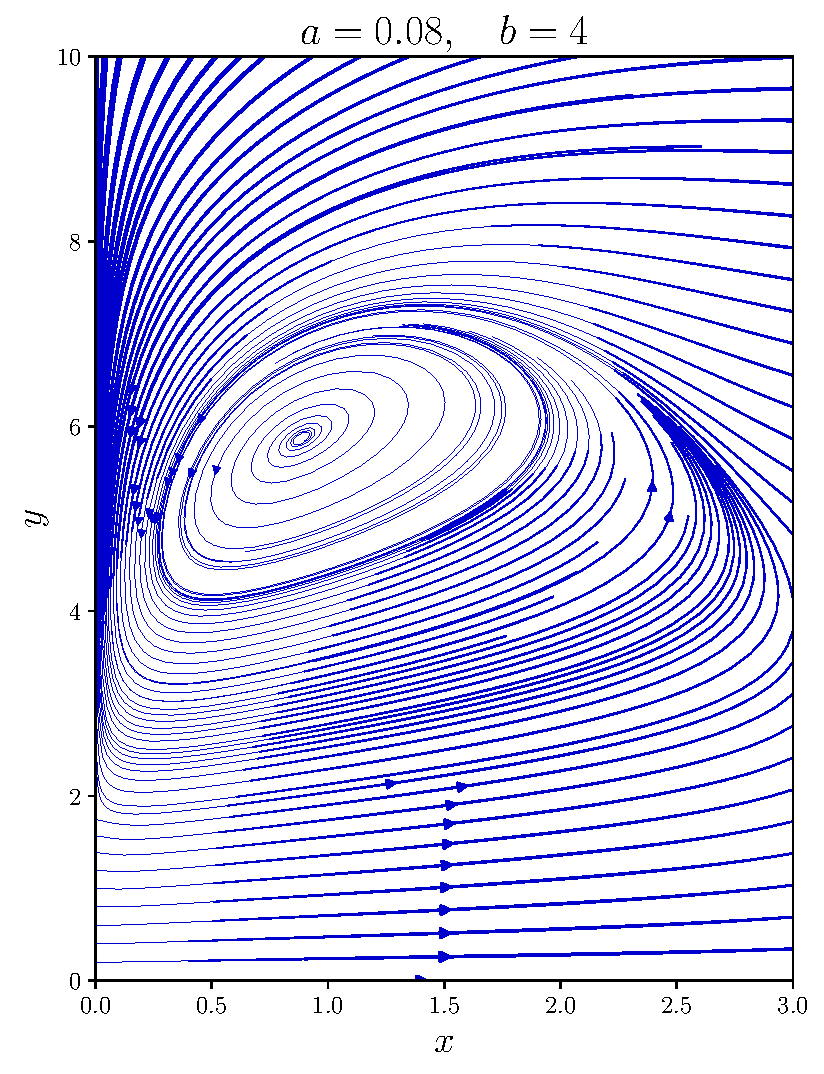
\includegraphics[width=\linewidth]{fig/8.2.9.overcrit}
		\caption{بالای نقطه بحرانی}
	\end{figure}
	\restoregeometry
	\begin{figure}[h!]
		\centering
		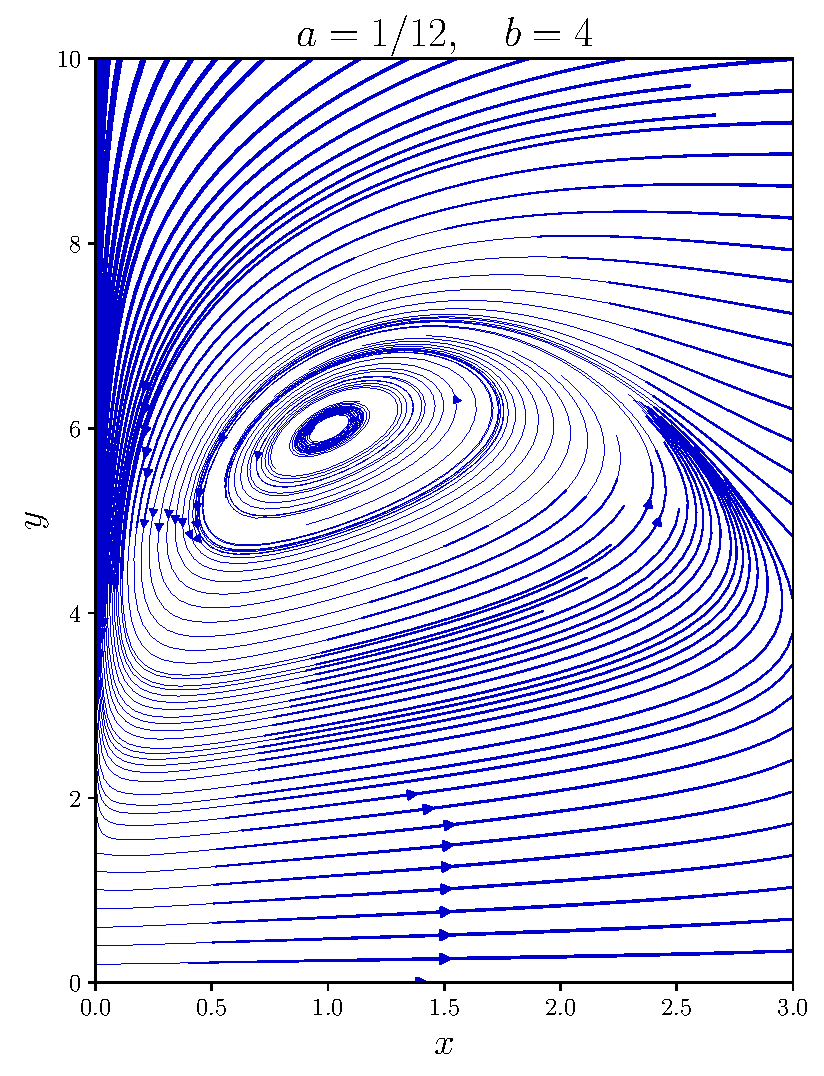
\includegraphics[width=\linewidth]{fig/8.2.9.critical}
		\caption{نقطه بحرانی}
	\end{figure}
	\begin{figure}[h!]
		\centering
		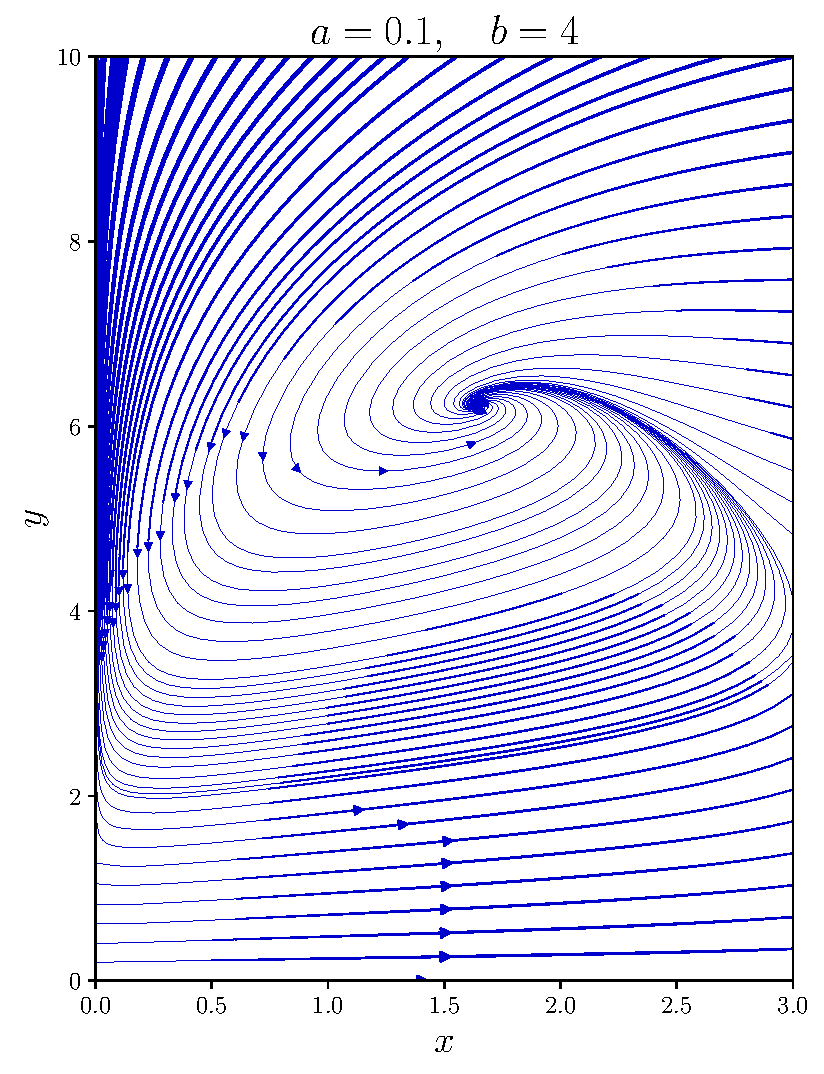
\includegraphics[width=\linewidth]{fig/8.2.9.undercrit}
		\caption{زیر نقطه بحرانی}
	\end{figure}
\end{document}